
\chapter{Diskrete Mathematik}

\section{Kombinatorik}

\subsection{Endliche Summen}

Problemstellungen der Kombinatorik führen oftmals zu Summen.
Ein Grund dafür liegt darin, dass die Lösungen bestimmter
Differenzengleichungen als Summen darstellbar sind. In der Analysis
sind die Reihen sehr bedeutsam, das sind Summen von unendlich vielen
Summanden. Der Wert einer Reihe wird hierbei, sofern existent, als der
Grenzwert der Folge der Partialsummen erklärt.
Somit bauen Reihen konzeptuell auf den endlichen Summen auf.
Ein weiteres wichtiges Werkzeug stellen die formalen Potenzreihen bereit,
die ohne den Grenzwertbegriff auskommen, aber analoge Rechenregeln zu
den eigentlichen Potenzreihen aufweisen. In der linearen Algebra dienen
Summen ebenfalls zur allgemeinen Formulierung von Rechenregeln.
Darin einbegriffen ist das Rechnen mit Polynomen. Auch in der
Stochastik sind Summen dienlich, zum Beispiel zur Erklärung des
Erwartungswertes einer Zufallsgröße.

Zur Einführung eine kleine Aufgabe. Man beobachtet
\[1+3 = 2^2,\quad 1+3+5 = 3^2,\quad 1+3+5+7 = 4^2,\quad 1+3+5+7+9 = 5^2.\]
Anscheinend besteht die Gesetzmäßigkeit
\[1 + 3 + \ldots  + (2n-1) = n^2.\]
In Worten ist die Summe der ersten ungeraden Zahlen eine Quadratzahl,
genauer die Anzahl der Summanden zum Quadrat. Ein strenger Beweis dafür
findet sich unschwer. Zuvor will ich aber die allgemeinen Gesetzmäßigkeiten
für das Rechnen mit Summen diskutieren.

Statt Summen mit drei Pünktchen zu beschreiben, verwendet man meist die
unmissverständliche Notation
\[\textstyle\sum_{k=1}^n a_k := a_1 + a_2 + \ldots + a_n.\]
Beispielsweise gilt
\[\textstyle\sum_{k=1}^3 (2k-1) =
(2\cdot 0-1) + (2\cdot 1 -1 ) + (2\cdot 2 - 1)
= 1 + 3 + 5.\]
Die drei Pünktchen treten allerdings noch in der Erklärung der Summe
auf. Wir werden sie wieder gänzlich los, indem die Summe rekursiv
festgelegt wird.

\begin{Definition}[Summe]\newlinefirst
Für eine Folge $a\colon\Z\to\R$ ist die \emph{Summe} der $a_k$ für $k=m$
bis $k=n$ rekursiv definiert gemäß
\[\sum_{k=m}^{m-1} a_k := 0,\quad \sum_{k=m}^n a_k := a_n + \sum_{k=m}^{n-1} a_k.\]
\end{Definition}
Es darf $k$, genannt der \emph{Laufindex}, als gebundene Variable nur
im Term $a_k$ auftreten. Die Zahlen $m,n$ nennt man die \emph{Grenzen}
der Summierung. Ist $a$ lediglich auf $D\subseteq\Z$ definiert, können
wir $a$ schlicht per $a_k := 0$ für $k\notin D$ auf ganz $\Z$ erweitern.
Dies bietet sich an, wenn die Summe stets definiert sein soll,
unabhängig davon wie die Grenzen gewählt werden.

\begin{Satz}\label{Summe-Homogenitaet}
Es gilt $\sum_{k=m}^n ca_k = c\sum_{k=m}^n a_k$ für jede Konstante $c$.
\end{Satz}
\begin{Beweis}
Induktion über $n$. Im Induktionsanfang $n=m-1$ gilt
\[\textstyle\sum\limits_{k=m}^{m-1} ca_k \stackrel{\mathrm{def}}= 0 = c\cdot 0
\stackrel{\mathrm{def}}= c\sum\limits_{k=m}^{m-1} a_k.\]
Der Induktionsschritt ist
\[\textstyle\sum\limits_{k=m}^n ca_k \stackrel{\mathrm{def}}= ca_n+\sum\limits_{k=m}^{n-1} ca_k
\stackrel{\mathrm{IV}}= ca_n + c\sum\limits_{k=m}^{n-1} a_k
= c\Big(a_n + \sum\limits_{k=m}^{n-1} a_k\Big) \stackrel{\mathrm{def}}= c\sum\limits_{k=m}^n a_k.\,\qedsymbol\]
\end{Beweis}

\begin{Satz}\label{Summe-Additivitaet}
Es gilt $\sum_{k=m}^n (a_k+b_k) = \sum_{k=m}^n a_k + \sum_{k=m}^n b_k$.
\end{Satz}
\begin{Beweis}
Induktion über $n$. Im Induktionsanfang $n=m-1$ reduziert sich die
Behauptung zu $0 = 0 + 0$. Der Induktionsschritt ist%
\begin{align*}
\textstyle\sum_{k=m}^n (a_k + b_k) &\textstyle\stackrel{\mathrm{def}}=
a_n + b_n + \sum_{k=m}^{n-1} (a_k + b_k)
\stackrel{\mathrm{IV}}=
a_n + b_n + \sum_{k=m}^{n-1} a_k + \sum_{k=m}^{n-1} b_k\\
&\textstyle\stackrel{\mathrm{def}}= \sum_{k=m}^n a_k + \sum_{k=m}^n b_k.\,\qedsymbol
\end{align*}
\end{Beweis}
Man kann den Raum $\Abb(\Z,\R)$ auch als einen Vektorraum über dem Körper
$\R$ deuten, wobei die Multiplikation mit einem Skalar $c\in\R$ und die
vektorielle Addition punktweise definiert werden, das heißt,%
\[(ca)_k := ca_k,\quad\; (a+b)_k := a_k+b_k.\]
Dann ist $\sum_m^n a := \sum_{k=m}^n a_k$ eine lineare Abbildung,
denn die Homogenität gilt laut Satz \ref{Summe-Homogenitaet}, und
die Additivität laut Satz \ref{Summe-Additivitaet}.

Der Differenzoperator
\[(\Delta a)_n := a_{n+1} - a_n\]
wird die nachfolgende Diskussion übersichtlicher halten. Es handelt
sich ebenfalls um eine lineare Abbildung, das heißt, für jede Konstante
$c$ und alle Folgen $a,b$ gilt $\Delta (ca) = c\Delta a$ und
$\Delta(a+b) = \Delta a + \Delta b$, denn%
\begin{align*}
(\Delta (ca))_n &= ca_{n+1} - ca_n = c(a_{n+1}-a_n) = c(\Delta a)_n,\\
(\Delta(a+b))_n &= (a_{n+1}+b_{n+1}) - (a_n + b_n)
= a_{n+1} - a_n + b_{n+1} - b_n\\
&= (\Delta a)_n + (\Delta b)_n.
\end{align*}

\begin{Satz}[Teleskopsumme]
Es gilt $\sum_{k=m}^{n-1} (\Delta a)_k = a_n - a_m$.
\end{Satz}
\begin{Beweis}
Induktion über $n$. Im Induktionsanfang $n=m$ sieht man trivial,
dass beide Seiten der Gleichung den Wert null haben. Der
Induktionsschritt ist%
\[\sum\limits_{k=m}^n (\Delta a)_k \stackrel{\mathrm{def}}=
(\Delta a)_n + \sum\limits_{k=m}^{n-1} (\Delta a)_k
\stackrel{\mathrm{IV}}= a_{n+1} - a_n + a_n - a_m = a_{n+1} - a_m.\,\qedsymbol\]
\end{Beweis}

\noindent
Das Prinzip der Teleskopsummen bietet zwei wesentliche Vorteile. 
Der erste Vorteil besteht darin, dass man damit bequem nach
Summenformeln fischen kann, wobei man deren Beweis mit geschenkt
bekommt. Für $s_n := (n-1)/n$ gilt zum Beispiel%
\[(\Delta s)_n = \frac{n}{n+1} - \frac{n-1}{n}
= \frac{n^2 - (n+1)(n-1)}{(n+1)n} = \frac{1}{(n+1)n}.\]
Ergo findet sich die Summenformel
\[\sum_{k=1}^n \frac{1}{(k+1)k} = \frac{n}{n+1}.\]
Der zweite Vorteil besteht darin, dass sich der Beweis einer bereits
ermittelten Summenformel dahingehend vereinfacht, dass nicht jedes
mal ein Induktionsbeweis geführt werden muss, womit die unter Umständen
schwierige Auffindung der wesentlichen Umformungen im Induktionsschritt
erleichtert wird. Zum Beweis einer Summenformel der Form%
\[\textstyle\sum_{k=1}^n a_k = s_{n+1} - s_1\]
genügt es nämlich, $\Delta s = a$ zu prüfen. Zur Summenformel%
\[\textstyle\sum_{k=1}^n (2k-1) = n^2\]
gilt beispielsweise $a_n = 2n-1$ und $s_n = (n-1)^2$. Es bestätigt sich
kurzerhand%
\[(\Delta s)_n = n^2 - (n-1)^2 = n^2 - n^2 + 2n - 1  = 2n-1 = a_n.\]
Aus der nun bewiesenen Formel ziehen sich schnell weitere Schlüsse.
Setzt man in die Gleichung%
\[\textstyle n^2 = \sum_{k=1}^n (2k-1) = 2\sum_{k=1}^n k - \sum_{k=1}^n 1\]
die Vereinfachung $\sum_{k=1}^n 1 = n$ ein und stellt sie daraufhin nach
der verbleibenden Summe um, findet sich die Summenformel%
\[\sum_{k=1}^n k = \frac{1}{2}(n^2 + n) = \frac{n}{2}(n+1).\]
Die Werte dieser Summe werden die \emph{Dreieckszahlen} genannt.%
\footnote{Engl. \emph{triangular numbers}. Eintrag A000217 in OEIS.}

\begin{Satz}[Aufteilung von Summen]%
\label{Summe-Aufteilung}\newlinefirst
Für $m\le p\le n$ gilt
$\sum_{k=m}^n a_k = \sum_{k=m}^{p-1} a_k+\sum_{k=p}^n a_k$.
\end{Satz}
\begin{Beweis}
Induktion über $n$. Der Induktionsanfang liege in $n=p$. Die Gleichung
ist in diesem erfüllt, weil $\sum_{k=p}^p a_k=a_p$ gilt.
Der Induktionsschritt ist%
\[\sum\limits_{k=m}^n a_k \stackrel{\mathrm{def}}= a_n+\sum\limits_{k=m}^{n-1} a_k
\stackrel{\mathrm{IV}}= a_n + \sum\limits_{k=m}^{p-1} a_k + \sum\limits_{k=p}^{n-1} a_k
\stackrel{\mathrm{def}}= \sum\limits_{k=m}^{p-1} a_k + \sum\limits_{k=p}^n a_k.\,\qedsymbol\]
\end{Beweis}

\begin{Satz}[Indexverschiebung]%
\label{Summe-Indexshift}\newlinefirst
Für die Indexverschiebung der Distanz $d\in\Z$,
kurz Indexshift, gilt\\
$\sum_{k=m}^n a_k = \sum_{k=m+d}^{n+d} a_{k-d}.$
\end{Satz}
\begin{Beweis}
Induktion über $n$. Im Induktionsanfang $n=m-1$ wird unmittelbar
ersichtlich, dass beide Seiten der Gleichung im Wert null resultieren.
Der Induktionsschritt gilt gemäß der Umformung%
\begin{align*}
\sum_{k=m}^n a_k \stackrel{\mathrm{def}}= a_n+\sum_{k=m}^{n-1} a_k
\stackrel{\mathrm{IV}}= a_{(n+d)-d}+\sum_{k=m+d}^{n+d-1} a_{k-d}
\stackrel{\mathrm{def}}= \sum_{k=m+d}^{n+d} a_{k-d}.\,\qedsymbol
\end{align*}
\end{Beweis}

\noindent
Ich will zusätzlich noch eine alternative Herleitung aufzeigen. Bei
dieser wird der Indexbereich als Ungleichung beschrieben, was den
Vorteil bietet, dass die Ungleichung einer Umformung unterzogen werden
kann. Mit der Substitution $k=k'-d$ gelingt dahingehend die Überlegung%
\begin{align*}
\sum_{k=m}^n a_k = \sum_{m\le k\le n} a_k
= \!\!\sum_{m\le k'-d\le n}\!\! a_{k'-d}
= \!\!\sum_{m+d\le k'\le n+d}\!\! a_{k'-d}
= \sum_{k'=m+d}^{n+d} a_{k'-d}.
\end{align*}

\begin{Satz}[Umkehrung der Reihenfolge]%
\label{Summe-Umkehrung}\newlinefirst
Es gilt $\sum_{k=0}^n a_k = \sum_{k=0}^n a_{n-k}$.
\end{Satz}
\strong{Beweis.}
Der Induktionsanfang bei $n=0$ ist trivial. Beim Induktionsschritt
macht man sich Satz \ref{Summe-Indexshift} (Indexshift) und
Satz \ref{Summe-Aufteilung} (Aufteilung) zunutze,%
\begin{gather*}
\sum_{k=0}^n a_{n-k} = a_{n-n}+\sum_{k=0}^{n-1} a_{n-k}
= a_0+\sum_{k=0}^{n-1} a_{n-(n-1-k)}
= a_0+\sum_{k=0}^{n-1} a_{k+1}\\
\stackrel{[k:=k-1]}= a_0+\sum_{k=1}^n a_k
= \sum_{k=0}^0 a_k + \sum_{k=1}^n a_k
= \sum_{k=0}^n a_k.\,\qedsymbol
\end{gather*}
Dienlich ist die Umkehrung beispielsweise bei der folgenden klassischen
Herleitung der Summenformel $\sum_{k=0}^n k = \tfrac{n}{2}(n+1)$. 
Aufbauend auf den bereits gezeigten Regeln stellt diese Herleitung ebenfalls
einen strengen Beweis dar. Das doppelte der Summe betrachtet man hierbei
als Addition der Summe zu sich selbst, wobei die Reihenfolge der zweiten
Summe umgekehrt wird. Man erhält%
\begin{align*}
2\sum_{k=0}^n k &= \sum_{k=0}^n k+\sum_{k=0}^n k
= \sum_{k=0}^n k + \sum_{k=0}^n (n-k)\\
&= \sum_{k=0}^n (k+n-k) = \sum_{k=0}^n n
= n\sum_{k=0}^n 1 = n(n+1).
\end{align*}
Ganz allgemein dürfen die Summanden einer endlichen Summe beliebig
umgeordnet werden; dies geht aus wiederholter Anwendung des Kommutativgesetzes
und des Assoziativgesetzes hervor. Die Formalisierung dieser Tatsache
geschieht vermittels einer frei wählbaren Permutation des Indexbereichs.
Der zuvor diskutierte Sachverhalt stellt sich dahingehend als
Spezialfall mit der auf der Menge $\{0,\ldots,n\}$ definierten
Permutation $\pi(k) = n-k$ dar.

\begin{Satz}[Permutation der Reihenfolge]%
\label{Summe-Permutation-Index}\newlinefirst
Sei $M=\{k\in\Z\mid m\le k\le n\}$. Für jede Permutation
$\pi\colon M\to M$ gilt
\[\sum_{k=m}^n a_k = \sum_{k=m}^n a_{\pi(k)}.\]
\end{Satz}
\begin{Beweis} Induktion über $n$. Sei ohne Beschränkung der Allgemeinheit $m=1$.
Im Induktionsanfang $n=0$ und $n=1$ ist die Gleichung offenkundig erfüllt.

Induktionsschritt. Induktionsvoraussetzung sei die Gültigkeit für $M$.
Zu zeigen ist die Gültigkeit für $M\cup\{n+1\}$.

Sei $t$ ein fester Parameter mit $1\le t\le n+1$.
Im Fall $\pi(t) = n+1$ geht man wie folgt vor.
Man setze $\sigma(k):=\pi(k)$ für $1\le k\le t-1$. Man setze
$\sigma(k):=\pi(k+1)$ für $t\le k\le n$. Weil $n+1$ kein Wert von
$\sigma$ ist, muss $\sigma$ eine Permutation $\sigma\colon M\to M$ sein.
Ergo gilt
\begin{align*}
\sum_{k=1}^{n+1} a_{\pi(k)} &= \sum_{k=1}^{t-1} a_{\pi(k)}
+ a_{\pi(t)} + \sum_{k=t+1}^{n+1} a_{\pi(k)}
= a_{\pi(t)} + \sum_{k=1}^{t-1} a_{\pi(k)}
+ \sum_{k=t}^n a_{\pi(k+1)}\\
&= a_{n+1} + \sum_{k=1}^{t-1} a_{\sigma(k)}
+ \sum_{k=t}^n a_{\sigma(k)}
= a_{n+1} + \sum_{k=1}^n a_{\sigma(k)}\\
&\stackrel{\mathrm{IV}}= a_{n+1} + \sum_{k=1}^n a_k
= \sum_{k=1}^{n+1} a_k.
\end{align*}
Man beachte, dass in den beiden Randfällen $t=1$ und $t=n+1$ die
jeweilige Randsumme den Wert null hat und somit verschwindet.\,\qedsymbol
\end{Beweis}

\noindent
Dass die Reihenfolge der Summierung keine Rolle spielt, gibt Anlass
zu einer abstrakten Fassung der Summierung selbst, die von vornherein
auf die Festlegung einer bestimmten Reihenfolge verzichtet.

\begin{Satz}
Sei $M$ eine endliche Menge, sei $a\colon M\to\R$. Die Festlegung
\[\sum_{k\in M} a_k := \sum_{i=m}^n a_{f(i)},\;\; |M| = n-m+1,\;\;
f\colon\{m,\ldots,n\}\to M\;\text{bijektiv}\]
ist wohldefiniert, wobei $f$ frei gewählt werden darf.
\end{Satz}
\begin{Beweis}
Es gilt zu zeigen, dass die Summe auch wirklich unabhängig von der
gewählten Bijektion ist. Sind $f,g$ zwei solcher Bijektionen, so ist
$\pi := g^{-1}\circ f$ ebenfalls bijektiv, also eine Permutation des
Indexbereichs. Vermittels Satz \ref{Summe-Permutation-Index} gilt daher
\[\sum_{i=m}^n a_{f(i)} = \sum_{i=m}^n a_{g(\pi(i))}
= \sum_{i=m}^n a_{g(i)}.\,\qedsymbol\]
\end{Beweis}

\noindent
Im Weiteren ist man nun befähigt, die Begrenzung des Indexbereichs
durch Ungleichungen streng zu definieren. Man legt fest
\[\sum_{m\le k\le n} a_k := \sum_{k\in M} a_k,
\quad M := \{k\in\Z\mid m\le k\land k\le n\}.\]
Somit ist streng begründet, dass die Ungleichungen $m\le k$
und $k\le n$ einer Äquivalenzumformung unterzogen werden dürfen,
denn von diesen bleibt die Menge $M$, und somit die Summe unberührt.

Ein letztes Detail darf aber nicht vergessen werden. Im Vorfeld der
oder Anschluss an die Umformung der Ungleichungen wird ggf. eine
Substitution der Laufvariable durchgeführt. Streng genommen muss noch
abgeklärt werden, dass dies unter allen Umständen unverfänglich ist.
Gewissheit schafft der

\begin{Satz}[Substitutionsregel]
Ist $\varphi\colon M'\to M$ eine Bijektion, gilt
\[\sum_{k\in M} a_k = \sum_{k'\in M'} a_{\varphi(k')}.\]
\end{Satz}
\begin{Beweis}
Zur Bijektion $f\colon\{1,\ldots,|M|\}\to M$ existiert die Bijektion
$g$ mit $f = \varphi\circ g$, nämlich ist dies $g:=\varphi^{-1}\circ f$.
Infolge gilt
\[\sum_{k\in M} a_k = \sum_{i=1}^{|M|} a_{f(i)}
= \sum_{i=1}^{|M|} a_{\varphi(g(i))}
= \sum_{k'\in M'} a_{\varphi(k')}.\,\qedsymbol\]
\end{Beweis}
Für die allgemeine Form der Summierung gelten anloge Regeln. Genauer
lassen sich die bereits bewiesenen Regeln direkt übertragen.
Man prüft unschwer nach, dass gilt
\[\sum_{k\in M} ca_k = c\sum_{k\in M}a_k,\qquad\sum_{k\in M} (a_k+b_k)
= \sum_{k\in M} a_k + \sum_{k\in M} b_k.\]
Zur Aufteilung sei $M = A\cup B$ mit $A\cap B = \emptyset$, also
eine disjunkte Zerlegung von $M$ in $A,B$. Dann gilt
\[\sum_{k\in M} a_k = \sum_{k\in A} a_k + \sum_{k\in B} a_k.\]
Bezüglich der Indikatorfunktion $1_A\colon M\to\{0,1\}$
zu $A\subseteq M$ gilt nun
\[\sum_{k\in M} 1_A(k)a_k = \sum_{k\in A} a_k,\]
denn $M=A\cup (M\setminus A)$ ist eine disjunkte Zerlegung, so dass gilt
\[\sum_{k\in M} 1_A(k)a_k = \sum_{k\in A} \underbrace{1_A(k)}_{=1}a_k
+ \sum_{k\in M\setminus A} \underbrace{1_A(k)}_{=0}a_k
= \sum_{k\in A} a_k.\]
Ist $A\subseteq\Z$ endlich, dürfen wir daher definieren
\[\sum_k 1_A(k)a_k = \sum_{k\in\Z} 1_A(k)a_k := \sum_{k\in A} a_k,\]
da diese Summe in Wirklichkeit endlich ist, also niemals über
unendlich viele Indizes läuft. Diese Sichtweise bietet unter Umständen
Vorteile bei der Umformung von Summen.

\subsection{Endliche Produkte}

Endliche Produkte weisen analoge Rechenregeln zu den endlichen Summen
auf, kommen allerdings weit weniger häufig vor als diese. Infolgedessen
verlaufen die Beweise ebenso analog, weshalb ich darauf verichten will,
diese weitläufig aufzuführen. Verbreitet sind endliche Produkte von
Zahlen vor allem in der Kombinatorik, zum Beispiel in Form von Faktoriellen
und Binomialkoeffizienten.

Für eine Folge $a\colon\Z\to\R$ definiert man rekursiv
\[\prod_{k=m}^{m-1} a_k := 1,\quad\;
\prod_{k=m}^n a_k := a_n\prod_{k=m}^{n-1} a_k.\]
Sei $c\in\Z_{\ge 0}$ eine Konstante. Es gilt
\[\prod_{k=m}^n a_k^c = \Big(\prod_{k=m}^n a_k\Big)^c,\qquad
\prod_{k=m}^n (a_k b_k) = \Big(\prod_{k=m}^n a_k\Big)\Big(\prod_{k=m}^n b_k\Big).\]
Die Aufteilung von Produkten geht vonstatten gemäß
\[\prod_{k=m}^n a_k = \Big(\prod_{k=m}^{p-1} a_k\Big)
\Big(\prod_{k=p}^n a_k\Big), \quad m\le p\le n+1.\]
Für jede Konstante $c\in\R$ gilt
\[\prod_{k=m}^n c = c^{n+1-m},\qquad
\prod_{k=m}^n (ca_k) = c^{n+1-m}\prod_{k=m}^n a_k.\]
Bei manchen Umformungen hilft das Teleskopprodukt
\[\prod_{k=m}^n\frac{a_{k+1}}{a_k} = \frac{a_{n+1}}{a_m},\quad
\text{sofern}\;\,\forall k\in\{m,\ldots,n\}\colon a_k\ne 0.\]

\subsection{Anzahl der Abbildungen}

Abstrakt gesehen thematisiert die abzählende Kombinatorik die Frage
nach der Anzahl der Elemente endlicher Mengen. Die Mengenlehre
hilft bei der Formalisierung, und infolgedessen beim strengen Beweis
kombinatorischer Gesetzmäßigkeiten.

Zur Einführung stellt man häufig die Frage, wie viele mögliche Tupel
eine Produktmenge enthält. Üblicherweise formuliert man diese
unkomplizierte Aufgabe aber nicht in der Gestalt der Mengenlehre,
sondern fragt, wie viele Zahlen eine Binärsequenz aus $k$ Bits enthält,
oder wie viele Zeichenketten der Länge $k$ mit 26 Buchstaben
formulierbar sind. Abstrakt gesehen geht es bei den Binärsequenzen um
die Anzahl der Elemente von $\{0,1\}^k$. Analog geht es bei den
Zeichenketten um die Anzahl der Elemente von
\[\{\verb|'a'|,\verb|'b'|,\ldots,\verb|'z'|\}^k.\]
Die Elemente sind jeweils Tupel der Länge $k$. Bezüglich $B^k$ will
ich $|B|$ so wie bei Stellenwertsystemen als die \emph{Basis}
bezeichnen. Dass $|A\times B| = |A|\cdot |B|$ für beliebige Mengen
gilt, wurde bereits aufgezeigt. Demnach gilt
\[|B^k| = |B|^k = n^k, \quad n:=|B|.\]
Mit den $n=2$ Binärwerten sind dies 256 Binärsequenzen der Länge $k=8$.
Oder mit $n=26$ Buchstaben sind es 676 Zeichenketten der Länge $k=2$,
und schon 17576 Zeichenketten der Länge $k=3$.

In der Vergangenheit empfahlen Dienste häufig oder machten es obligatorisch,
Passwörter dadurch sicherer zu machen, indem neben Buchstaben auch noch
Ziffern und Sonderzeichen eingegeben werden sollten. Man
empfahl also, die Basis $n$ zu vergrößern, um die Länge gering zu halten.
Nimmt man an, dass so ein Passwort rein zufällig ausgewürfelt wird, ist
es bei bereits hinreichend großer Basis aber wesentlich sinnvoller,
abermals den Exponenten $k$ zu erhöhen. Bei Hinzunahme der 10 Ziffern zu
den 26 Buchstaben bekommt man mit $n=36$ für $k=3$ eine Zahl von 46656
Zeichenketten. Unterscheidet man zudem zwischen kleinen und großen
Buchstaben, sind es immerhin 238328. Mit $n=26$ und $k=4$ sind es aber
bereits 456976.

In der professionellen Kryptografie nennt man $n^k$ die
\emph{Schlüsselraumgröße}, die bei modernen symmetrischen Kryptosystemen
mindestens $2^{128}$ beträgt. Und der Schlüssel wird am besten rein
zufällig gewählt. Zur Kodierung in der Basis $n$ muss man die Gleichung
$2^{128} = n^k$ nach $k$ umformen, das macht
\[k = 128\,\tfrac{\mathrm{lg}(2)}{\mathrm{lg}(n)}.\]
Das sind acht Blöcke je vier Hexadezimalziffern. Oder 22 Zeichen
zur Basis 62. Es ist davon auszugehen, dass dies ebenso sehr ein sicheres
Passwort darstellt.

Zur Erinnerung, ein Tupel aus $B^k$ darf auch als eine endliche Folge
interpretiert werden, das ist eine Abbildung
$\{0,\ldots,k-1\}\to B.$
Dahingehend ergibt sich die abstrakte Fassung

\begin{Satz}[Anzahl der Abbildungen]\label{Anzahl-Abb}\newlinefirst
Seien $X,Y$ endliche Mengen mit $|X| = k$ und $|Y|=n$. Die Menge
der Abbildungen $X\to Y$ enthält $n^k$ Elemente.
\end{Satz}
\begin{Beweis}
Induktion über $k$. Im Anfang $k=0$ ist $X=\emptyset$. Es gibt genau
eine Abbildung $\emptyset\to Y$, nämlich die leere Abbildung.
Gleichermaßen ist $n^0=1$.

Zum Induktionsschritt. Induktionsvoraussetzung sei die Gültigkeit
für $k-1$. Es  sei $|X|=k$ und $|Y|=n$. Gesucht ist die Anzahl
der Möglichkeiten zur Festlegung der Abbildung $f\colon X\to Y$.
Sei $x\in X$ fest. Für die Festlegung $f(x)=y$ bestehen nun genau $n$
Möglichkeiten, nämlich so viele, wie es Elemente $y\in Y$ gibt.
Die Festlegung der übrigen Werte geschieht gemäß der Einschränkung
von $f$ auf $X\setminus\{x\}$, und die Zahl dieser Abbildungen beträgt
$n^{k-1}$ gemäß der Induktionsvoraussetzung. Man hat also $n$ mal
$n^{k-1}$ Möglichkeiten, das sind $n^k$.\,\qedsymbol
\end{Beweis}
Gleichwohl die dargelegte Beweisführung recht genau erscheint,
bezieht sie sich im Induktionsschritt an der wesentlichen Stelle
auf rationale Überlegungen, die allerdings nicht aus bereits
formal bewiesenen Regeln der Mengenlehre entstammen. Zur Schließung der
Lücke muss man sich daran erinnern, dass
\[|Y^{A\cup B}| = |Y^A\times Y^B| = |Y^A|\cdot |Y^B|,\;
\text{sofern}\; A\cap B=\emptyset.\]
Zusammen mit $|Y^{\{x\}}|=n$ wird der Induktionsschritt damit präzisiert zu
\[|Y^X| = |Y^{(X\setminus\{x\})\cup\{x\}}| = |Y^{X\setminus\{x\}}|\cdot |Y^{\{x\}}|
\stackrel{\mathrm{IV}}= n^{k-1}\cdot n = n^k.\]

\subsection{Anzahl der Injektionen}

Bei den Passwörtern durfte jedes Zeichen beliebig oft vorkommen.
Stellt man die Aufgabe so, dass jedes Zeichen nur ein einziges
Mal vorkommen darf, verringert sich die Anzahl der Möglichkeiten.
Zum Beispiel wird gefragt nach der Zahl der Ketten, die aus zwei der
vier Buchstaben $\mathrm{a,b,c,d}$ besteht. Man kann dazu ein Baumdiagramm
aufstellen. Für den ersten Buchstaben bestehen vier Möglichkeiten,
woraufhin für den zweiten Buchstaben jeweils noch drei Möglichkeiten
übrig bleiben. Das macht $4\cdot 3 = 12$ Möglichkeiten.
Die Berechnung verläuft gemäß der

\begin{Definition}[Fallende Faktorielle]\newlinefirst
Für $n\in\Z$ und $k\in\Z_{\ge 0}$ legt man rekursiv fest
\[n^{\underline 0} := 1,\quad\;
n^{\underline k} := n\cdot (n-1)^{\underline{k-1}}.\]
\end{Definition}

\noindent
Zu $n=4$ Buchstaben und $k=2$ Stellen ergibt sich
\[n^{\underline k} = 4^{\underline 2} = 4\cdot 3^{\underline 1}
= 4\cdot 3\cdot 2^{\underline 0} = 4\cdot 3\cdot 1 = 12.\]
Per Induktion über $k$ bestätigt man die Produktformel
\[n^{\underline k} = \prod_{i=0}^{k-1} (n-i) = \prod_{i=1}^k (n+1-i)
= n\cdot (n-1)\cdot\ldots\cdot (n+1-k).\]
Der Sachverhalt kann nun wieder abstrakt gefasst werden.

\begin{Satz}[Anzahl der Injektionen]\newlinefirst
Seien $X,Y$ endliche Mengen, wobei $|X|=k$ und $|Y|=n$ gelte.
Die Menge der Injektionen $X\to Y$ enthält $n^{\underline k}$
Elemente.
\end{Satz}
\begin{Beweis}
Induktion über $k$. Im Anfang $k=0$ ist $X=\emptyset$. Es gibt
genau eine Injektion $\emptyset\to Y$, nämlich die leere Abbildung.
Gleichermaßen gilt $n^{\underline 0} = 1$.

Zum Schritt. Voraussetzung sei die Gültigkeit
für $k-1$. Es sei $|X|=k$ und $|Y|=n$. Gesucht ist die Anzahl
der Möglichkeiten zur Festlegung der Injektion $f\colon X\to Y$.
Sei $x\in X$ fest. Für die Festlegung $f(x)=y$ bestehen genau
$n$ Möglichkeiten, nämlich so viele, wie es Elemente $y\in Y$ gibt.
Bei der Festlegung der übrigen entfällt $y$ aufgrund der Injektivität
von $f$. Für die Festlegung betrachtet man $f$ daher als Injektion%
\[f\colon X\setminus\{x\}\to Y\setminus\{y\},\]
von denen es laut Voraussetzung $(n-1)^{\underline{k-1}}$ gibt. Es sind
also $n$ mal $(n-1)^{\underline{k-1}}$ Möglichkeiten, was definitionsgemäß
gleich $n^{\underline k}$ ist.\,\qedsymbol
\end{Beweis}

\noindent
Im Spezialfall $n=k$ muss müssen die Abbildungen außerdem surjektiv, und
damit bijektiv sein. Deren Anzahl wird gezählt durch die spezielle
fallende Faktorielle $n^{\underline n}$, die man \emph{Fakultät} nennt
und $n!$ notiert. Spezialisiert man die Definition der fallenden
Faktoriellen dahingehend, ergibt sich die
\begin{Definition}[Fakultät]\newlinefirst
Für $n\in\Z_{\ge 0}$ legt man rekursiv fest
\[0! := 1,\quad\; n! := n\cdot (n-1)!.\]
\end{Definition}
Speziell im Fall $X=Y$ sind die Bijektionen die Permutationen auf der
Menge $X$. Somit ist $n!$ auch die Anzahl der Permutationen von $n$
verschiedenen Objekten. In Alltagssprache formuliert lassen sich
$n$ unterschiedliche Gegenstände in $n!$ Reihenfolgen bringen.

\subsection{Anzahl der Teilmengen}

Aber wie verhält es sich, wenn die Reihenfolge keine Rolle spielt?
Dazu sei eine Menge $Y$ von $n=|Y|$ Objekten gegeben, aus der $k$ Objekte
ausgewählt werden. Diese Auswahl nennt man eine \emph{Kombination}.
Sie ist als Ansammlung unterschiedlicher Objekte, bei der es nicht auf
die Reihenfolge ankommt, aber wesensmäßig nichts anderes als eine Menge.
Gesucht ist demzufolge die Anzahl der Teilmengen von $Y$, die genau
$k$ Elemente enthalten. Die Lösung dieser Aufgabe wird berechnet durch
den \emph{Binomialkoeffizient} $\binom{n}{k}$, der zunächst einmal
erklärt werden muss.
\begin{Definition}[Binomialkoeffizent]\newlinefirst
Für $n\in\Z$ und $k\in\Z_{\ge 0}$ setzt man
\[\binom{n}{k} := \frac{1}{k!}n^{\underline k}.\]
\end{Definition}

\noindent
Stellt man den Binomialkoeffizent als Funktion von $(n,k)$ tabellarisch
dar, erkennt man früher oder später, dass dieser einer einfachen
Rekurrenz genügt. Nämlich liegt, insofern $n$ die Zeilen und $k$ die Spalten
durchläuft, die Summe zweier Einträge unterhalb des
zweiten Eintrags; die graphische Darstellung dieses Sachverhaltes wird
\emph{pascalsches Dreieck} genannt. Das heißt, es gilt der
\begin{Satz}
Für $n\in\Z$ und $k\ge 1$ gilt
\[\binom{n}{k} = \binom{n-1}{k-1} + \binom{n-1}{k}.\]
\end{Satz}
\begin{Beweis}
Es findet sich die Umformung
\begin{align*}
\hspace{-12pt}\binom{n-1}{k-1} + \binom{n-1}{k}
&= \frac{(n-1)^{\underline{k-1}}}{(k-1)!} + \frac{(n-1)^{\underline k}}{k!}
= \frac{k(n-1)^{\underline{k-1}}}{k!} + \frac{(n-1)^{\underline{k-1}}(n-k)}{k!}\\
&= \frac{(n-1)^{\underline{k-1}}}{k!}(k + n -k)
= \frac{n(n-1)^{\underline{k-1}}}{k!}
= \frac{n^{\underline k}}{k!} = \binom{n}{k}.\,\qedsymbol
\end{align*}
\end{Beweis}

\noindent
Setzt man die beiden Anfangsbedingungen $\binom{n}{0} = 1$ und $\binom{n}{n}=1$
zusätzlich voraus, wird $\binom{n}{k}$ für $0\le k\le n$ durch die
Rekurrenz charakterisiert. Genau genommen muss dafür zudem abgesichert
werden, dass die Rekursion zu jedem Argument $(n,k)$ durch die
Anfangsbedingungen fundiert ist, was aber leicht ersichtlich wird.
Da $n$ bei der Rekurrenz in jedem Argument um eins verringert
auftritt, wird aufgrund $0\le k\le n$ irgendwann $k=0$ oder $k=n$
sein müssen, weil sich der Abstand zwischen 0 und $n$ immer weiter vermindert.

\begin{Satz}[Anzahl der Teilmengen]\newlinefirst
Sei $Y$ eine $|Y|=n$ Elemente enthaltende endliche Menge und $C_k(Y)$
die Menge der $k$-elementigen Teilmengen von $Y$.
Es gilt $|C_k(Y)| = \binom{n}{k}$.
\end{Satz}
\begin{Beweis}
Induktion über $(n, k)$. Im Anfang ist $k=0$ oder $k=n$. Der abstruse
Fall $k=0$ sucht nach Teilmengen ohne Elemente. Es existiert genau eine
solche Menge, nämlich die leere Menge, womit $C_0(Y)=1$ ist. Der Fall
$k=n$ sucht nach Teilmengen, die so viele Elemente haben wie $Y$.
Dies kann nur $Y$ selbst sein, womit $C_n(Y)=1$ gilt.
Gleichermaßen gilt $\binom{n}{0}=1$ und $\binom{n}{n}=1$.

Induktionsvoraussetzung sei die Gültigkeit für $(n-1, k-1)$ und
$(n-1, k)$. Man nimmt nun ein Element $y$ aus $Y$ heraus,
womit darin $n-1$ verbleiben. Entscheidet man sich,
$y$ zur Teilmenge hinzuzufügen, verbleiben noch $k-1$ Elemente
auszuwählen. Entscheidet man sich dagegen, verbleibt die Teilmenge
unverändert, womit nach wie vor $k$ Elemente auszuwählen sind.
Die Anzahl der Möglichkeiten ist somit
\[|C_k(Y)| = |C_{k-1}(Y\setminus\{y\})| + |C_k(Y\setminus\{y\})|
\stackrel{\mathrm{IV}}=\binom{n-1}{k-1} + \binom{n-1}{k}
= \binom{n}{k}.\,\qedsymbol\]
\end{Beweis}

\begin{figure}\setlength{\abovecaptionskip}{0pt}
\begin{center}
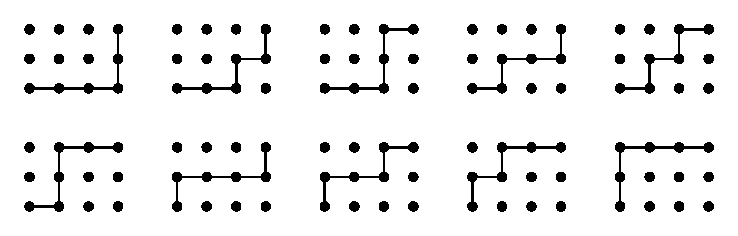
\includegraphics[width=125mm]{img/Gitterwege.pdf}
\caption{Die 10 monotonen Gitterwege von $(0,0)$ nach $(3,2)$.}
\label{fig:Gitterwege}
\end{center}
\end{figure}

\noindent
Kombinatorische Aufgaben tendieren dazu, sich einer bildlichen
Anschauung zu entziehen. Um dem ein wenig entgegenzuwirken, will
ich den folgenden Sachverhalt aufführen, der die Binomialkoeffizienten
mit monotonen Gitterwegen in Beziehung setzt. Als Beispiel listet
Abb. \ref{fig:Gitterwege} jeden der 10 möglichen Wege von Knoten
$(0,0)$ nach Knoten $(3,2)$ auf.

\begin{Satz}
Ein Weg auf dem Gitter $\Z\times\Z$ heiße \emph{monoton}, wenn von $(x,y)$
aus lediglich der Schritt nach $(x+1,y)$ oder der Schritt nach $(x,y+1)$
gewährt ist. Die Anzahl der monotonen Gitterwege von $(0,0)$ nach
$(x,y)$ beträgt
\[\frac{(x+y)!}{x!y!} = \binom{x+y}{x} = \binom{x+y}{y}.\]
\end{Satz}
\begin{Beweis}
Es bezeichne $f(x,y)$ die Anzahl der monotonen Wege von $(0,0)$ nach
$(x,y)$. Zum Erreichen eines Punktes auf den Achsen besteht immer
nur ein möglicher Weg, womit $f(x,0)=1$ und $f(0,y)=1$ gelten muss. Ein
nicht auf den Achsen befindlicher Punkt $(x,y)$ kann von $(x-1,y)$ oder
$(x,y-1)$ aus erreicht werden, was zur Rekurrenz
\[f(x,y) = f(x-1,y) + f(x,y-1)\]
führt. Die Tabellierung der Werte macht ersichtlich, dass sie
ein gedrehtes pascalsches Dreieck erzeugt. Wir setzen daher
$C(x+y,x):=f(x,y)$ und führen die Koordinatentransformation $x+y=n$
und $x=k$ aus. Die Rekurrenz nimmt damit die Form
\[C(n,k) = C(n-1,k-1) + C(n-1,k),\quad C(n,0)=1,\quad C(n,n)=1\]
an, die aber eindeutig den Binomialkoeffizienten charakterisiert.\,\qedsymbol
\end{Beweis}

\noindent
Ein analoger Sachverhalt besteht für Gitter in höheren Dimensionen,
was zum Begriff des \emph{Multinomialkoeffizienten} führt.

Man kann auch eine gruppentheoretische Sichtweise auf die Kombinationen
einnehmen. Die Teilmengen von $Y$ mit $k$ Elementen sind wie Listen, die
jedes der $k$ Elemente genau einmal enthalten. Der Unterschied zu diesen
Listen besteht genau darin, dass es bei den Teilmengen nicht auf die
Reihenfolge der Elemente ankommt. Um die Anzahl der Teilmengen zu
zählen, müssen demzufolge Listen, die sich lediglich durch ihre
Reihenfolge unterscheiden, als äquivalent angesehen werden. Ihre
Äquivalenzklassen stellen somit quasi Listen dar, die die Reihenfolge
ihrer Elemente vergessen haben.

Wir verwenden eine beliebige Menge $X$ mit $|X|=k$ als Indexmenge,
beispielsweise direkt $X:=\{0,\ldots,k-1\}$. Je zwei Listen sind damit
gegeben durch Injektionen $f,g\colon X\to Y$. Die beiden Listen werden
als äquivalent angesehen, sofern sie sich lediglich durch eine
Permutation $\pi$ ihrer Indizes unterscheiden, also
\[f\sim g\,:\Leftrightarrow\,\exists\pi\in S_k\colon f = g\circ\pi.\]
Es sei ferner $\mathrm{Inj}(X,Y)$ die Menge der Injektionen $X\to Y$
und $\mathrm{Inj}(X,Y)/S_k$ die Quotientenmenge bezüglich der
Äquivalenzrelation bzw. der Gruppe $S_k$.
\begin{Satz}\label{Bij-Inj-Teilmengen}
Es sei $C_k(Y)$ die Menge der $k$-elementigen Teilmengen von $Y$.
Zwischen $\mathrm{Inj}(X,Y)/S_k$ und $C_k(Y)$ besteht eine
kanonische Bijektion.
\end{Satz}
\begin{Beweis}
Wir definieren diese Bijektion als
\[\varphi\colon\mathrm{Inj}(X,Y)/S_k\to C_k(Y),\quad\varphi([f]) := f(X),\]
wobei $[f]=f\circ S_k$ die Äquivalenzklasse des Repräsentanten $f$
bezeichne. Die Abbildung $\varphi$ ist wohldefiniert, denn für je zwei $f,g$
mit $f\sim g$ ist eine Permutation $\pi$ vorhanden, so dass gilt
\[f(X) = (g\circ\pi)(X) = g(\pi(X)) = g(X).\]
Zum Nachweis der Injektivität von $\varphi$ muss $[f]=[g]$ aus
$f(X)=g(X)$ gewonnen werden. Gesucht ist also eine Permutation
$\pi$ mit $f=g\circ\pi$. Weil $g$ injektiv ist, existiert eine
Linksinverse $g^{-1}$, so dass $\pi := g^{-1}\circ f$ gewählt werden
kann. Es verbleibt die Gleichheit $f = g\circ g^{-1}\circ f$ zu
bestätigen. Zwar ist $g^{-1}$ im Allgemeinen keine Rechtsinverse von $g$,
ihre Einschränkung auf $g(X)$ aber schon. Wegen $f(X)=g(X)$ hebt sich
$g\circ g^{-1}$ daher auf $f(X)$ weg.

Zur Surjektivität von $\varphi$. Hier ist zu zeigen, dass es zu jeder
Menge $B\in C_k(Y)$ eine Injektion $f\colon X\to Y$ mit $f(X)=B$ gibt.
Weil $X$ und $B$ gleichmächtig sind, existiert eine Bijektion $f_0\colon X\to B$,
womit man die gesuchte Injektion mit der Setzung $f(x):=f_0(x)$ erhält.\,\qedsymbol
\end{Beweis}

\noindent
Bezüglich $|X|=k$ tut sich nun die Umformung
\[|C_k(Y)| \stackrel{\text{(1)}}= |\mathrm{Inj}(X,Y)/S_k|
\stackrel{\text{(2)}}= \frac{|\mathrm{Inj}(X,Y)|}{|S_k|} =
\frac{n^{\underline k}}{k!} = \binom{n}{k}\]
auf. Der Schritt (1) wurde bereits durch Satz
\ref{Bij-Inj-Teilmengen} abgeklärt. Die Einsicht in (2) erhält man
folgendermaßen. Für jede Gruppe $G$ gilt die Bahnformel
$|G| = |f\circ G|\cdot |G_f|$. Bei trivialer Fixgruppe $G_f$ gilt
$|G_f| = 1$, mithin $|f\circ G| = |G|$. Namentlich bei der symmetrischen
Gruppe $G=S_k$ tritt dieser Umstand ein. Aus diesem Grund enthält jede
Bahn $f\circ S_k$ gleich viele Elemente, $|S_k|$ an der Zahl. Weil
die Bahnen außerdem paarweise disjunkt sind, ergibt sich deshalb
die Faktorisierung
\[|\mathrm{Inj}(X,Y)| = |S_k|\cdot |\mathrm{Inj}(X,Y)/S_k|.\]
Der gemachte Gedankengang kann auch unter anderen Umständen vorgenommen
werden, dergestalt dass statt den Injektionen die Surjektionen oder sämtliche
Abbildungen betrachtet werden. Es entsteht der \emph{zwölffaltige Weg},
-- wenn man so will, ein kleines Periodensystem der Kombinatorik, 
siehe Tabelle \ref{tab:twelvefold-way}. \cite{Stanley}

\begin{table}
\begin{center}
\caption{Der zwölffaltige Weg}
\label{tab:twelvefold-way}
\begin{tabular}{c|ccc}
\toprule
& $f\in\Abb(X,Y)$ & $f\in\mathrm{Inj}(X,Y)$ & $f\in\mathrm{Sur}(X,Y)$\\
\midrule[\heavyrulewidth]
$f$ & $n^k$ & $n^{\underline k}$ & $n!\big\{\!\begin{smallmatrix}k\\ n\end{smallmatrix}\!\big\}$\\[4pt]
$f\circ S_k$ & $\big(\!\begin{smallmatrix}n+k-1\\ k\end{smallmatrix}\!\big)$
& $\big(\!\begin{smallmatrix}n\\ k\end{smallmatrix}\!\big)$
& $\big(\!\begin{smallmatrix}k-1\\ k-n\end{smallmatrix}\!\big)$\\[4pt]
$S_n\circ f$ & $\sum_{i=0}^n \big\{\!\begin{smallmatrix}k\\ i\end{smallmatrix}\!\big\}$
& $[k\le n]$ & $\big\{\!\begin{smallmatrix}k\\ n\end{smallmatrix}\!\big\}$\\[4pt]
$S_n\circ f\circ S_k$ & $p_n(n+k)$ & $[k\le n]$ & $p_n(k)$\\
\bottomrule
\end{tabular}
\end{center}
\end{table}

Der Term $\big\{\!\begin{smallmatrix}k\\ n\end{smallmatrix}\!\big\}$
steht dabei für die Stirlingzahlen zweiter Art, das ist die Anzahl der
Möglichkeiten, wie eine Menge von $k$ Elementen in $n$ disjunkte nichtleere
Teilmengen zerlegt werden kann. Der Term $p_n(k)$ steht für die Anzahl
der Partitionen der Zahl $k$ in $n$ Teile. Der Term $[k\le n]$ steht
für »$1$, falls $k\le n$, sonst $0$«.

\subsection{Anzahl der Multimengen}

Aus der Frage nach der Anzahl Kombinationen geht als abgewandelte
Problemstellung die Frage nach der Anzahl Kombinationen mit
Wiederholung einher. Das heißt, während bei einer Kombination von
$k$ aus $n$ unterschiedlichen Objekten jedes der $k$ Objekte höchstens
einmal auftreten darf, kann bei einer Kombination mit Wiederholung
jedes der $n$ Objekte beliebig häufig, also bis zu $k$ mal auftreten.
Während eine Kombinationen eine Menge von $k$ aus einer Menge von $n$
Elementen darstellt, handelt es sich bei einer Kombination mit
Wiederholung um eine Multimenge von $k$ aus der Menge von $n$ Elementen.

Eine gute Veranschaulichung bietet die folgende Aufgabe.
Aus einem Sack mit unerschöpflich vielen Bauklötzen der Farben rot, grün,
blau und gelb werden gleichzeitig fünf Stück gezogen. Zur Frage steht,
wie viele unterschiedliche Farbkombinationen es gibt.

\begin{figure}\setlength{\abovecaptionskip}{0pt}
\begin{center}
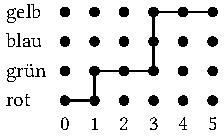
\includegraphics[width=38mm]{img/Kloetze.pdf}
\caption{Eine Kombination von fünf Klötzen in bis zu vier Farben.}
\label{fig:Kloetze}
\end{center}
\end{figure}

Diese Aufgabe kann als die Frage nach der Anzahl monotoner Gitterwege
umgedeutet werden. Ein Schritt nach rechts fügt dabei einen Klotz zur
Sammlung hinzu. Ein Schritt nach oben wechselt dagegen in die nächste Farbe,
ohne die bisherige Sammlung von Klötzen zu vergrößern.
Siehe Abb. \ref{fig:Kloetze}. Es stellt sich heraus, dass sich diese Sichtweise
zur Methodik \emph{Stars and Bars} gleichbedeutend verhält. Dabei wird
ein Sternchen für einen Klotz gesetzt und ein Stab als Abgrenzung
zwischen zwei Farben. Man setzt ein Sternchen also gerade für einen
Schritt nach rechts und einen Stab suggestiv für einen Schritt
nach oben.

Man muss hier vorsichtig sein, keinen Off-by-one-Fehler zu machen.
Zwar gibt es vier Farben, diese werden allerdings mit $0$, $1$, $2$, $3$
nummeriert. Eine Sammlung von $k$ Klötzen aus einem Sack mit $n$ Farben
entspricht also einem Gitterweg von $(0,0)$ zu $(k,n-1)$. Die Anzahl
der Farbkombinationen beträgt somit
\[\left(\!\left(\begin{matrix}n\\ k\end{matrix}\right)\!\right) :=
\binom{k+n-1}{k} = \binom{k+n-1}{n-1} = \binom{5+4-1}{4-1} = \binom{8}{3} = 56.\]
Das doppelt geklammerte Analogon zum Binomialkoeffizienten wird also als
die Anzahl der $k$-elementigen Multimengen mit Elementen aus einer Menge
von $n$ Elementen interpretiert. Wie es scheint, stimmt sie mit der Anzahl
der $k$-elementigen Teilmengen aus einer Menge von $k+n-1$ Elementen
überein.

\subsection{Gesamtzahl der Teilmengen}

Die Zählung der Teilmengen beschränkte sich zuvor auf Teilmengen fester
Größe. Nun würden wir gerne auch in Erfahrung bringen, wie viele mögliche
Teilmengen einer Menge $M$ es insgesamt gibt, also wie groß die
Potenzmenge von $M$ ist.

Zunächst kurz ein leichter Hilfssatz.

\begin{Satz}\label{ohne-ist-monoton}
Aus $A\subseteq B$ folgt $A\setminus C\subseteq B\setminus C$.
\end{Satz}
\begin{Beweis}
Es gelte $x\in A\setminus C$. Das bedeutet, $x\in A$ und $x\notin C$.
Laut der Voraussetzung folgt $x\in B$ aus $x\in A$. Somit gilt sowohl
$x\in B$ als auch $x\notin C$, also $x\in B\setminus C$.\,\qedsymbol
\end{Beweis}

\noindent
Als nächstes klären wir die Rekurrenz der Potenzmengenoperation ab,
die daraufhin in einem Induktionsbeweis Verwendung findet. Auf Basis
ihrer lässt sich außerdem ein Algorithmus zur Aufzählung der Potenzmenge
erstellen.

\begin{Satz}[Rekurrenz der Potenzmengenoperation]%
\label{Potenzmenge-rekursiv}\newlinefirst
Für $x\notin M$ gilt $\powerset(M\cup\{x\})
= \powerset(M)\cup\{A\cup\{x\}\mid A\in\powerset(M)\}$.
\end{Satz}
\begin{Beweis}
Die Gleichung ist äquivalent zu
\[T\subseteq M\cup\{x\}\,\Leftrightarrow\, T\subseteq M\lor\exists A\subseteq M\colon T=A\cup\{x\}.\]
Die rechte Seite gelte. Im Fall $T\subseteq M$ gilt erst
recht $T\subseteq M\cup\{x\}$. Im anderen Fall liegt ein $A\subseteq M$
vor, womit $A\cup\{x\}\subseteq M\cup\{x\}$ gilt. Wegen $T=A\cup\{x\}$
gilt also ebenfalls $T\subseteq M\cup\{x\}$.

Die linke Seite gelte. Mit $T\subseteq M\cup\{x\}$ und
$x\notin M$ folgt per Satz \ref{ohne-ist-monoton}
\[T\setminus\{x\}\subseteq (M\cup\{x\})\setminus\{x\} = M,
\;\text{also}\; T\setminus\{x\}\subseteq M.\]
Im Fall $x\notin T$ ist
$T=T\setminus\{x\}$, womit man $T\subseteq M$
erhält. Im gegenteiligen Fall $x\in T$ wird $A:=T\setminus\{x\}$
als Zeuge der Existenzaussage gewählt.\,\qedsymbol
\end{Beweis}

\noindent
Es verhält sich dergestalt, dass \emph{sämtliche} in der Rekurrenz
auftretende Vereinigungen solche disjunkter Mengen sind. Man darf
die Rekurrenz somit auch als
\[\powerset(M\uplus\{x\})
= \powerset(M)\uplus\biguplus_{\mathclap{A\in\powerset(M)}}
\{A\uplus\{x\}\}\]
notieren. Nun zur gesuchten Anzahl.

\begin{Satz}\label{Anzahl-Potenzmenge}
Mit $|M|=n$ gilt $|\powerset(M)| = 2^n$.
\end{Satz}
\begin{Beweis}
Induktion über $n$. Im Anfang $n=0$ muss $M=\emptyset$ sein, also
$\powerset(M)=\{\emptyset\}$, das macht $|\powerset(M)| = 1 = 2^0$.

Zum Schritt. Es gelte $|M|=n$ und es sei $x\notin M$. Vermittels Satz
\ref{Potenzmenge-rekursiv}, wo man es außerdem mit Vereinigungen
disjunkter Mengen zu tun hat, erhält man
\[|\powerset(M\cup\{x\})| = |\powerset(M)| + |\{A\cup\{x\}\mid A\in\powerset(M)\}|
\stackrel{\text{IV}}= 2^n + 2^n = 2^{n+1}.\,\qedsymbol\]
\end{Beweis}

\noindent
Einen kürzeren Beweis erhalten wir, wenn ihr uns daran erinnern, dass
$\powerset(M)$ und $\Abb(M,\{0,1\})$ gleichmächtig sind. Demnach gilt
\[|\powerset(M)| = |\Abb(M,\{0,1\})| = |\{0,1\}|^{|M|} = 2^{|M|}.\]
Als Korollar ergibt sich kurzerhand die Beziehung
\[\sum_{k=0}^n\binom{n}{k} = 2^n,\]
denn summiert man die Anzahl der $k$"=elementigen Teilmengen über $k$,
erhält man die Anzahl sämtlicher Teilmengen einer Menge von $n$ Elementen.
Und führt man einen unabhängigen Induktionsbeweis dieser Beziehung,
erhält man umgekehrt einen dritten Beweis von Satz \ref{Anzahl-Potenzmenge}.

\newpage
\section{Zur elementaren Zahlentheorie}

\subsection{Kongruenzen}

Die elementare Zahlentheorie beschäftigt sich mit der Teilbarkeit von
Zahlen, den Resten, die bei der Ganzzahldivision übrig bleiben
und der Auffindung ganzzahliger Lösungen von Gleichungen. Lange Zeit
als ein Gebiet der reinen Mathematik angesehen, stellte sie sich
als bedeutsam für die praktische Informatik und die Kryptologie heraus. 

Die \emph{modulare Arithmetik}, auch \emph{Restklassenarithmetik}
genannt, ist ein wichtiges Hilfsmittel der elementaren Zahlentheorie.
Sie geht aus der gewöhnlichen Arithmetik hervor, indem zwei ganze
Zahlen als gleich angesehen werden, wenn sie bei Division durch eine
vorab gewählte feste Zahl denselben Rest lassen. Diese Form der
Gleichheit nennt man \emph{Kongruenz}, die feste Zahl den \emph{Modul}.
Kongruenz zweier Zahlen ist damit gleichbedeutend, dass die eine
Zahl zur anderen um ein Vielfaches des Moduls verschoben liegt, was nichts
anderes bedeutet, als dass der Modul die Differenz der beiden Zahlen teilt.

Man vermittelt das Konzept gern am Lauf von Uhrzeigern. Hierbei werden
die Stunden $0, 12, 24, 36$ usw. als gleich angesehen. Entsprechend
werden die Stunden $1, 13, 25, 37$ usw. als gleich angesehen. Es
verbleiben nur noch $12$ unterschiedliche Zeitpunkte, die vollen
Stunden $0, 1, \ldots, 11$. Ein Uhrzeiger auf $11$ Uhr trifft
zwei Stunden später auf $1$ Uhr. Anders ausgedrückt sind die Zahlen
$11+2$ und $1$ kongruent Modulo 12, was nach Carl Friedrich Gauß
in der Form
\[11 + 2\equiv 1\pmod{12}\]
notiert wird.

\begin{Definition}[Kongruenz]\index{Kongruenz}\newlinefirst
Zwei ganze Zahlen $a,b$ heißen kongruent modulo $m$, wenn ihre Differenz
$a-b$ durch $m$ teilbar ist,%
\[a\equiv b\pmod{m}\;:\Leftrightarrow\;\exists k\in\Z\colon a-b=km.\]
\end{Definition}
Statt »$(\mathrm{mod}\;m)$« schreibt man beim Rechnen meist
kürzer »$(m)$«.

\begin{Satz}
Die Kongruenz ist eine Äquivalenzrelation, das heißt, es gilt
\begin{align*}
&a\equiv a\pmod{m},&&\text{(Reflexivität)}\\
&a\equiv b\cond b\equiv a\pmod{m},&&\text{(Symmetrie)}\\
&a\equiv b\land b\equiv c\cond a\equiv c\pmod{m}.&&\text{(Transitivität)}
\end{align*}
\end{Satz}
\begin{Beweis}
Für die Reflexivität ist ein $k$ mit $0=a-a=km$
zu finden. Setze $k=0$.

Bei der Symmetrie gibt es nach Voraussetzung
ein $k$ mit $a-b=km$. Dann ist $b-a=-km$. Setze $k'=-k$.
Es gibt also $k'$ mit $b-a=k'm$, somit gilt $b\equiv a$.

Bei der Transitivität gibt es nach Voraussetzung ein $k$ mit
$a-b=km$ und ein $l$ mit $b-c=lm$. Das heißt, es gilt
$km+lm = a-c$, \text{ergo} $a-c = (k+l)m$. Setze $k'=k+l$. Es gibt also
$k'$ mit $a-c=k'm$. Somit gilt $a\equiv c$.\;\qedsymbol
\end{Beweis}

\begin{Satz}\label{Kongruenz-add-sub}
Für ganze Zahlen $a,b,c$ gelten die Äquivalenzen
\begin{align*}
a\equiv b\pmod{m}&\;\Leftrightarrow\; a+c\equiv b+c\pmod{m},\\
a\equiv b\pmod{m}&\;\Leftrightarrow\; a-c\equiv b-c\pmod{m}.
\end{align*}
\end{Satz}
\begin{Beweis}
Unter Beachtung von $(b+c)-(a+c)=b-a$ findet man
\begin{align*}
a\equiv b\pmod{m}
&\iff (\exists k\in\Z\colon b-a=km)\\
&\iff (\exists k\in\Z\colon (b+c)-(a+c)=km)\\
&\iff a+c\equiv b+c\pmod{m}.
\end{align*}
Bei der Subtraktion von $c$ verläuft die Überlegung analog.\;\qedsymbol
\end{Beweis}

%\newpage
\begin{Satz}\label{Kongruenz-mul}
Für ganze Zahlen $a,b,c$ gilt die Implikation
\[a\equiv b\pmod{m} \;\Rightarrow\; ac\equiv bc\pmod{m}.\]
\end{Satz}
\begin{Beweis}
Unter der Voraussetzung $a\equiv b\pmod{m}$ gibt es ein
$k$ mit $b-a=km$. Es gilt im Weiteren die Umformung
\[b-a=km\iff (b-a)c=kcm \iff bc-ac=k'm\]
mit $k':=kc$. Man hat also $\exists k'\in\Z\colon bc-ac=k'm$, was
definitionsgemäß äquivalent zu $ac\equiv bc\pmod{m}$ ist.\;\qedsymbol
\end{Beweis}

\begin{Satz}
Gilt $a\equiv a'\pmod{m}$ und
$b\equiv b'\pmod{m}$, dann gilt auch
\begin{align*}
a+b&\equiv a'+b'\pmod{m},\\
a-b&\equiv a'-b'\pmod{m},\\
ab&\equiv a'b'\pmod{m}.
\end{align*}
\end{Satz}
\strong{Beweis.} Es findet sich:
\[\begin{array}{@{}l@{\qquad\quad}l@{}}
\begin{prooftree}
    \hypo{a\equiv a'}
  \infer1{a+b\equiv a'+b}
    \hypo{b\equiv b'}
  \infer1{a'+b\equiv a'+b'}
\infer2{a+b\equiv a'+b'}
\end{prooftree}
&
\begin{prooftree}
    \hypo{a\equiv a'}
  \infer1{ab\equiv a'b}
    \hypo{b\equiv b'}
  \infer1{a'b\equiv a'b'}
\infer2{ab\equiv a'b'}
\end{prooftree}
\end{array}\]
Alle Kongruenzen sind hier modulo $m$ für $m$ fest, aber beliebig. Für
die Subtraktion verläuft die Überlegung analog.\qedsymbol

\begin{Satz}
Addition des Moduls führt auf eine kongruente Zahl:%
\[a\equiv a+m\equiv a-m\pmod{m}.\]
\end{Satz}
\begin{Beweis}
Es gilt
\[a\equiv a+m\pmod{m}\iff (\exists k\in\Z\colon km=(a+m)-a=m).\]
Man setze $k=1$. Bei
\[a\equiv a-m\pmod{m}\iff (\exists k\in\Z\colon km=(a-m)-a=-m)\]
setze man $k=-1$.\;\qedsymbol
\end{Beweis}

\subsection{Teilbarkeit}

Die Beziehung »$m$ teilt $a$« ist definiert als
\[m\mid a\;:\Leftrightarrow\; (\exists k\in\Z\colon a=km)
\;\Leftrightarrow\; a\equiv 0\pmod{m}.\]
Während die Kongruenz eine Äquivalenzrelation ist, stellt die
Teilbarkeit eine Halbordnung dar, dergestalt dass sie die drei Axiome
\begin{align*}
&\forall a\in\Z\colon a\mid a, &&\text{(Reflexivität)}\\
&\forall a,b\in\Z\colon a\mid b\land b\mid a\cond a = b,&&\text{(Antisymmetrie)}\\
&\forall a,b,c\in\Z\colon a\mid b\land b\mid c\cond a\mid c.&&\text{(Transitivität)}
\end{align*}
erfüllt. Teilt $a$ die Zahl $b$, ist $a$ also in gewisser Weise kleiner
als oder gleich $b$.

\subsection{Restklassenringe}

Wir könnten nun beginnen, mit der modularen Arithmetik interessante
Probleme zu lösen. Zunächst möchte ich aber erläutern, wie die
modulare Arithmetik mit dem Restklassenring zusammenhängt. Unter
diesem Blickwinkel bekommen wir ein tieferes Verständnis und können
Mittel der Ringtheorie und Gruppentheorie anwenden.

Zu einer ganzen Zahl $a$ ist die \emph{Restklasse}\index{Restklasse}
modulo $m$ definiert als 
\[[a]_m := \{x\mid x\equiv a\pmod m\}.\]
Eine alternative Schreibweise für $[a]_m$ ist $a+m\Z$. Weil die
Kongruenz eine Äquivalenzrelation ist, handelt es sich bei den
Restklassen um Äquivalenzklassen. Wir betrachten nun die
Quotientenmenge
\[\Z/m\Z := \{[a]_m\mid a\in\Z\}.\]
Nun können wir die Addition und Multiplikation von Restklassen
definieren.
\begin{Satz}
Auf $\Z/m\Z$ sind die beiden Operationen
\begin{align*}
[a]_m + [b]_m &:= [a+b]_m,\\
[a]_m\cdot [b]_m &:= [ab]_m
\end{align*}
wohldefiniert.
\end{Satz}
\strong{Beweis.} Zu zeigen ist, dass $a+b\equiv x+y$ gilt, sofern
$a\equiv x$ und $b\equiv y$ ist. Gemäß Satz \ref{Kongruenz-add-sub} gilt
\begin{align*}
a\equiv x &\iff a+b\equiv x+b,\\
b\equiv y &\iff x+b\equiv x+y.
\end{align*}
Aus den beiden Prämissen erhalten wir demzufolge
$a+b\equiv x+b\equiv x+y$.
Die Argumentation zur Multiplikation ist analog, wobei
Satz \ref{Kongruenz-mul} zur Anwendung kommt.\,\qedsymbol

Die Struktur $(\Z/m\Z,+,\cdot)$ nennt man den \emph{Restklassenring}%
\index{Restklassenring} zum Modul $m$.

\begin{Satz}
Jeder Restklassenring ist ein kommutativer unitärer Ring.
\end{Satz}
\begin{Beweis}
Bereits bewiesen wurde, dass die ganzen Zahlen einen
kommutativen unitären Ring bilden. Aufgrund der Wohldefiniertheit der
Addition und Multiplikation ist Kongruenz modulo $m$ eine
Kongruenzrelation. Satz \ref{Kongruenz-Ring-Quotient} zeigt somit die
Behauptung.\,\qedsymbol
\end{Beweis}

\noindent
Zudem ist die Quotientenabbildung
\[\varphi\colon\Z \to \Z/m\Z,\quad \varphi(a):=[a]_m.\]
ein Eins-erhaltender Ringhomomorphismus, wie aus dem Beweis
von Satz \ref{Kongruenz-Ring-Quotient} hervorgeht.

%\newpage
\subsection{Euklidische Division}

\begin{Satz}[Lemma zur euklidischen Division]\mbox{}\\*
Zu je zwei ganzen Zahlen $a,b$ mit $b\ne 0$ gibt es zwei eindeutig
bestimmte Zahlen $q,r$ mit $0\le r<|b|$, so dass $a=bq+r$. Man nennt
$q$ den \emph{Quotient} und $r$ den \emph{Rest}.
\end{Satz}
\begin{Beweis}[Beweis der Existenz]
Betrachten wir zunächst den Fall, bei dem $a\ge 0$
und $b>0$ ist. Man kann dann sooft $b$ von $a$ abziehen, bis sich eine
Zahl $\ge 0$ und $<b$ ergibt. Formal bilden wir die
Folge $r_k := a-bk$. Nun muss für irgendein $k\ge 0$ schließlich
$0\le r_k<b$ sein. Damit ist $q=k$ und $r=r_k$ gefunden.

Sei nun $a<0$. Wie bereits gezeigt gibt es $q,r$ mit $-a = bq+r$.
Für $r=0$ haben wir dann mit $q':=-q$ und $r':=0$ einen Quotient
und einen Rest. Sei nun $r\ne 0$. Dann gilt
\[a = -bq-r = -(q+1)b + b - r.\]
Mit $q':=-(q+1)$ und $r':=b-r$ gibt es somit auch in diesem Fall einen
Quotient und einen Rest. Der Rest erfüllt auch die gewünschte
Ungleichung, denn aus $r<b$ ergibt sich $0<r'$ und aus $0<r$ ergibt
sich $r'<b$.

Sei nun $a$ beliebig und $b<0$. Dann gibt es $q,r$ mit $a=(-b)q+r$.
Setze also $q':=-q$ und $r':=r$. Damit gilt $a=bq'+r'$, womit
auch in diesem Fall ein Quotient und ein Rest gefunden ist.\,\qedsymbol
\end{Beweis}
\begin{Beweis}[Beweis der Eindeutigkeit]
Das Paar $q,r$ erfülle
$a=bq+r$ und $q',r'$ erfülle ebenfalls $a=bq'+r'$. Dann gilt
\[bq+r = bq'+r',\iff b(q-q') = r'-r,\implies |b| |q-q'| = |r'-r|.\]
Aus $0<r<|b|$ und $0<r'<|b|$ erhält man außerdem $|r'-r|<|b|$. Somit
muss $|b| |q-q'| < |b|$ sein, also $|q-q'| < 1$. Eine nichtnegative
ganze Zahl kann aber nur dann kleiner als eins sein, wenn sie null
ist. Damit hat man
\[|q-q'|=0,\iff q-q'=0,\iff q=q'.\]
Entsprechend folgt $r=r'$.\,\qedsymbol
\end{Beweis}

Bei der euklidischen Division $a:b$ ist $(a\bmod b)$ eine geläufige
Schreibweise für den Rest. Das Lemma zur euklidischen Division sagt uns,
dass jede Restklasse von $\Z/m\Z$ einen kanonischen Repräsentant
besitzt. Nämlich besitzt die Restklasse $[a]_m$ den kanonischen
Repräsentant $r=(a\bmod m)$, denn $a=mq+r$ bedeutet dass $a-r$ durch
$m$ teilbar ist, also
\[a\equiv r\pmod m,\quad\text{bzw.}\quad [a]_m = [r]_m.\]


\subsection{Rundung}

Manche Formeln oder Rechnungen verlangen das Runden von Zahlen auf
eine ganze Zahl oder auf eine bestimmte Zahl von Nachkommastellen.
Im Algorithmus, der Vektorgrafiken als Rastergrafik aus Pixeln rendern
soll, muss zum Beispiel zwangsläufig an irgendeiner Stelle gerundet
werden. Außerdem ist Runden in vielen händischen Rechnungen
allgegenwärtig, sei es in wissenschaftlichen, technischen, gewerblichen
oder alltäglichen.

Als nächstes will ich daher erklären, wie Funktionen zum Runden formal
definiert werden, und welche Eigenschaften sie besitzen. Als wichtige
Grundfunktionen treten dabei die \emph{Abrundungsfunktion}, engl.
\emph{floor}, und die \emph{Aufrundungsfunktion}, engl. \emph{ceil},
auf, die vereinzelt auch in der Kombinatorik und in der Zahlentheorie
vorkommen.

\begin{Definition}[Floor]\label{def:floor}\index{Floorfunktion}
Für $x\in\R$ definiert man
\[y = \lfloor x\rfloor\,:\Leftrightarrow\, y\in\Z\land 0\le x-y < 1.\]
\end{Definition}

\begin{Definition}[Ceil]\label{def:ceil}\index{Ceilfunktion}
Für $x\in\R$ definiert man
\[y = \lceil x\rceil\,:\Leftrightarrow\, y\in\Z\land 0\le y-x < 1.\]
\end{Definition}

\begin{Satz}\label{floor-add-int}
Für jede ganze Zahl $k$ gilt $\lfloor k + x\rfloor = k + \lfloor x\rfloor$.
\end{Satz}
\begin{Beweis} Aufgrund der Prämisse $k\in\Z$ ist $y\in\Z$ äquivalent
zu $y-k\in\Z$. Unter dieser Gegebenheit findet sich mit
Def. \ref{def:floor} die äquivalente Umformung
\begin{align*}
y = \lfloor k+x\rfloor &\iff y\in\Z\land 0\le (k+x)-y < 1\\
&\iff y-k\in\Z\land 0\le x-(y-k) < 1\\
&\iff y - k = \lfloor x\rfloor \iff y = k + \lfloor x\rfloor.\,\qedsymbol
\end{align*}
\end{Beweis}

\begin{Satz}\label{floor-is-zero}
Für $0\le x < 1$ gilt $\lfloor x\rfloor = 0$.
\end{Satz}
\begin{Beweis}
Dies folgt unmittelbar aus Def. \ref{def:floor}.\,\qedsymbol
\end{Beweis}

\begin{Satz}
Es gilt
\[\begin{array}{@{}l@{\,}c@{\,}c@{}l@{\,}c@{\,}c@{}l}
\lfloor x\rfloor &=& \max &\{k\in\Z\mid k\le x\} &=& \min &\{k\in\Z\mid x < k + 1\},\\[2pt]
\lceil x\rceil &=& \min &\{k\in\Z\mid x\le k\} &=& \max &\{k\in\Z\mid k - 1 < x\}.
\end{array}\]
\end{Satz}
\begin{Beweis}
Mit bezüglich $y=\lfloor x\rfloor$ entfalteten Def. \ref{def:floor},
\ref{def:max-min} lautet die Aussage
\[y\in\Z\land 0\le x-y<1\;\Leftrightarrow\;
y\in\Z\land y\le x\land (\forall k\in\Z\colon k\le x\cond k\le y).\]
Für die Implikation von links nach rechts ist im Wesentlichen
\[k\in\Z, y\in\Z, k\le x, x < y+1\vdash k\le y\]
zu zeigen. Man erhält zunächst $k < y+1$ per Transitivgesetz.
Wegen $k,y\in\Z$ folgt daraus $k\le y$. Für die Implikation von rechts
nach links ist im Wesentlichen
\[y\in\Z,(\forall k\in\Z\colon k\le x\cond k\le y)\vdash x < y + 1\]
zu zeigen. Angenommen, es wäre $y+1\le x$. Die Allaussage wird mit
$k:=y+1$ spezialisiert. Per Modus ponens erhält man den Widerspruch
$y+1\le y$. Ergo muss die Annahme falsch sein, was äquivalent zu
$x<y+1$ ist. Die restlichen Beweise verlaufen analog.\,\qedsymbol
\end{Beweis}

\begin{Satz}\label{floor-div-floor}
Für $x\in\R$ und $n\in\Z_{\ge 1}$ gilt
\[\left\lfloor\frac{x}{n}\right\rfloor
= \left\lfloor\frac{\lfloor x\rfloor}{n}\right\rfloor.\]
\end{Satz}
\begin{Beweis}
Sei $a:=x-\lfloor x\rfloor$. Per Def. \ref{def:floor} gilt $0 \le a < 1$.
Laut dem Lemma zur euklidischen Division gilt außerdem
$\lfloor x\rfloor = qn+r$
mit $q=\lfloor\frac{\lfloor x\rfloor}{n}\rfloor$
und $0\le r\le n - 1$. Infolge gilt $0\le a+r<n$, also
$0\le\frac{a+r}{n}<1$ und somit $\lfloor\frac{a+r}{n}\rfloor = 0$
laut Satz \ref{floor-is-zero}.
Es findet sich%
\[\left\lfloor\frac{x}{n}\right\rfloor
= \left\lfloor\frac{a+\lfloor x\rfloor}{n}\right\rfloor
= \left\lfloor\frac{a+qn+r}{n}\right\rfloor
\stackrel{\text{(1)}}= q + \left\lfloor\frac{a+r}{n}\right\rfloor
\stackrel{\text{(2)}}= q =
\left\lfloor\frac{\lfloor x\rfloor}{n}\right\rfloor,\]
wobei (1) laut Satz \ref{floor-add-int} gilt, und (2)
wie soeben ausgeführt.\,\qedsymbol
\end{Beweis}

\begin{Satz}
Für $x\in\R$ und $m,n\in\Z$ mit $n\ge 1$ gilt
\[\left\lfloor\frac{m+x}{n}\right\rfloor
= \left\lfloor\frac{m+\lfloor x\rfloor}{n}\right\rfloor.\]
\end{Satz}
\begin{Beweis}
Laut Satz \ref{floor-add-int} ist $m+\lfloor x\rfloor = \lfloor m+x\rfloor$.
Die Aussage folgt nun als Korollar aus Satz \ref{floor-div-floor}.\,\qedsymbol
\end{Beweis}

\noindent
Das Runden einer Zahl auf eine ganze Zahl kann vermittels floor als
\[\mathrm{round}(x) := \mathrm{sgn}(x)\lfloor |x|+\tfrac{1}{2}\rfloor\]
beschrieben werden. Das Runden auf die $n$-te Nachkommastelle daraufhin als
\[\mathrm{round}(x, n) := \frac{\mathrm{round}(10^n x)}{10^n}.\]
